\documentclass[11pt]{article}
\usepackage{preamble}
\title{A Mori–Zwanzig memory kernel for subglacial drainage: the surge-lag memory is hydraulic, not ice-thermal}
\author{Abdelrahman Saifelden\\ Alexandria Higher Institute of Engineering and Technology (AIET), Alexandria, Egypt\\ \texttt{Abdulrahman.Saifelden22011411@aiet.edu.eg}}
\date{\today}
\begin{document}
\maketitle

\emph{Abdelrahman Saifelden (AIET) — Abdulrahman.Saifelden22011411@aiet.edu.eg}


\begin{abstract}


Post-drainage ice-stream speed-ups lag their subglacial trigger by months to a couple of years, and the lag carries \emph{memory}: the response rises to a peak rather than decaying monotonically. We make one claim and defend it three ways. \textbf{The lumped, linearised cavity\ensuremath{\leftrightarrow}channel storage system's surge response is an exact Mori–Zwanzig memory kernel}: projecting out the channel variable yields a generalized Langevin equation whose kernel equals the eliminated subsystem's own Green's function (verified to $7\times 10^{-18}$, projection exact to $5\times 10^{-16}$, reduced model reproducing the full trajectory to $9\times 10^{-8}$), with the Markovian (adiabatic-elimination) local closure recovered exactly as the channel time vanishes. This certifies \emph{why} surge response carries memory and \emph{how} it degenerates to a local closure — a structural result, not a field-validated lag value. We motivate it by \textbf{falsifying the only zeroth-order alternative}: a literal ice-thermal lag $\tau _{ice}=H^{2}/\kappa _{ice}$ is rejected by \textasciitilde{}5 orders of magnitude on the 131 Siegfried \& Fricker (2018) active lakes (median $\tau _{ice}\approx 1.5\times 10^{5} yr$ vs observed 0.02–2 yr; robust on the independent Arthern et al. (2015) thickness inversion, $r=0.970$), and on first principles (the thermal skin depth at surge periods is metres, and an impulse gives a peakless $t^{-1/2}$ response while observations peak). We then expose the kernel to the one open co-temporal dataset — a matched lake-drainage\ensuremath{\to}velocity test (CryoSat-2 drainage dates + ITS\_LIVE speeds) — which returns an \textbf{honest null} (peak $+0.56\sigma $, 0/5 significant), limited by temporal aliasing and an amplitude bound, not record precision, with two concrete unblock routes. Finally we include, as a continental \emph{screen} rather than a forecast, the Regime Transition Number $RTN$, show it is by construction the flotation/effective-pressure ratio (so a constant-$\phi $ $RTN$ adds no skill over thickness-above-flotation), and identify its only genuine degree of freedom — a spatially-varying basal-connectivity fraction $\phi (x,y)$ — with a plant-and-recover proof and a real-Bedmap2 hydraulic-routing demonstration. The contributions are the exact MZ certification (with two extensions that retire the ``it is just a 2\ensuremath{\times}2 linear-algebra identity'' objection: a \emph{nonlinear} extension — the linear kernel is the small-amplitude limit of the Röthlisberger system, which predicts that bigger floods lag longer; and a \emph{distributed} extension — the kernel is an exact, spatially non-local operator projection of the linearised flowline PDE whose no-transport, single-node limit is exactly the lumped 2\ensuremath{\times}2, and which predicts a finite along-flow memory footprint), the honest-falsifier discipline, and the diagnosis of the matched-lag null — not a verified surge-lag value.


\end{abstract}


\section*{1. Introduction}


Subglacial hydrology controls ice-stream sliding through the effective pressure $N=p_{i}-p_{w}$, the difference between ice overburden and basal water pressure (Cuffey \& Paterson 2010; Schoof 2010; Röthlisberger 1972). Drainage events — subglacial-lake floods — perturb $N$ and trigger transient speed-ups (Stearns et al. 2008; Siegfried et al. 2016), but the speed-up \emph{lags} the drainage and the lagged response is non-monotone (it peaks), implying the cavity\ensuremath{\leftrightarrow}channel system carries memory (Werder et al. 2013; Hewitt 2013). The modelling question is what sets that memory.


The mainstream tools are established and we use, not claim, them: the Mori–Zwanzig/Nakajima–Zwanzig projection and the generalized Langevin equation (Mori 1965; Nakajima 1958; Zwanzig 1960, 1973), the Röthlisberger channel and GlaDS-type cavity\ensuremath{\leftrightarrow}channel drainage (Röthlisberger 1972; Werder et al. 2013; Hewitt 2013), and the flotation/effective-pressure criterion (Schoof 2007; Leguy et al. 2014). What is new here is not a mechanism but an \textbf{exact structural certification} and the \textbf{discipline applied to its alternatives}.


\textbf{What is new, stated against the closest prior work.} Werder/Hewitt model the cavity\ensuremath{\leftrightarrow}channel system forward; we instead \emph{reduce} its linearisation by exact projection and show the surge-lag memory kernel \textbf{is} the eliminated channel subsystem's Green's function, with the local (Markovian) closure recovered as a limit — a closed-form statement of \emph{why} the lag has memory and \emph{when} a local sliding closure is admissible. No established theory predicts the literal $H^{2}/\kappa $ thermal lag; we state it as an explicit straw hypothesis precisely so the active-lake record can reject it, and report that rejection as a \emph{motivated null} rather than a discovery.


\textbf{Contributions.}

\begin{enumerate}
\item A \textbf{motivated falsification} of the literal $H^{2}/\kappa $ ice-thermal sliding-lag kernel on 131 real lakes, relocating the memory into hydrology (§3).
\item The \textbf{exact Mori–Zwanzig structure} of the cavity\ensuremath{\leftrightarrow}channel hydraulic memory kernel — a structural certification (§4), with a \textbf{nonlinear extension} showing the linear kernel is the small-amplitude limit of the physical Röthlisberger system and predicting an amplitude-dependent (bigger-floods-lag-longer) surge lag (§4.4), and a \textbf{distributed (spatially-resolved) extension} showing the kernel is an exact operator projection of the linearised flowline PDE — the lumped 2\ensuremath{\times}2 is its no-transport, single-node limit, and channel transport gives the surge-lag memory a finite along-flow footprint (§4.5).
\item An \textbf{honest matched-lag null} with a precise account of \emph{why} it is null (aliasing + amplitude bound, not noise) and two routes to a verified lag (§5).
\item A nondimensional \textbf{intrusion screen} $RTN$, shown to equal the flotation ratio, with its only genuine degree of freedom (a data-derived $\phi (x,y)$) isolated and tested (§6) — presented as a screen, not a verified forecast.
\item \textbf{Calibrated estimators} via synthetic plant-and-recover (§7).
\end{enumerate}


\medskip\hrule\medskip


\section*{2. Data and methods}


\begin{center}\small
\begin{tabularx}{\linewidth}{>{\raggedright\arraybackslash}X>{\raggedright\arraybackslash}X>{\raggedright\arraybackslash}X}
\toprule
Dataset & What & Access \\
\midrule
BAS \textbf{Bedmap2} & thickness, bed, surface, grounded mask (1 km) & open, no auth \\
\textbf{USAP-DC 601470} (Stubblefield et al. 2021) & independent thickness (Arthern et al. 2015) + 131 lake stats & open (USAP-DC) \\
\textbf{BedMachine v4} (NSIDC-0756) & independent continental thickness (RTN screen) & NSIDC (Earthdata) \\
\textbf{Siegfried \& Fricker (2018)} & 131 active subglacial-lake outlines & open (GitHub mirror) \\
\textbf{ITS\_LIVE} & surface-speed datacubes (image-pair $v$) & open (anonymous S3) \\
\textbf{CryoSat-2} in-lake elevation & drainage \emph{dates} & open (Siegfried 2021-GRL mirror) \\
\textbf{USAP-DC 601439} & ICESat lake volume-change (drainage volumes) & open \\
\bottomrule
\end{tabularx}
\end{center}


Runners raise \code{DataUnavailableError} with provisioning hints rather than fabricate gated series. Synthetic harnesses (\code{validation/\allowbreak{}synthetic/\allowbreak{}}) are exercised in \code{pytest} and prove the math against controlled inputs.


\medskip\hrule\medskip


\section*{3. The thermal sliding-lag kernel, falsified}


\textbf{3.1 The hypothesis (a motivated null).} No established sliding theory predicts that surge lag equals the \emph{full-thickness} ice thermal-diffusion time; we state $\tau _{ice} = H^{2}/\kappa _{ice}$ ($\kappa _{ice}=1.09\times 10^{-6} m^{2} s^{-1}$) as an explicit, falsifiable straw hypothesis precisely so the data can reject it.


\textbf{3.2 The test.} On real Bedmap2 thickness at the 131 Siegfried \& Fricker (2018) catalogued active lakes (130 with valid thickness; median $H=2282 m$, range 637–3905 m):


\begin{itemize}
\item $\tau _{ice} = H^{2}/\kappa _{ice}$: \textbf{median \ensuremath{\approx} 1.5\ensuremath{\times}10\ensuremath{^{5}} yr} (p5 \ensuremath{\approx} 2\ensuremath{\times}10\ensuremath{^{4}}; p95 \ensuremath{\approx} 3\ensuremath{\times}10\ensuremath{^{5}} yr).
\item Observed post-drainage surge lags: \textbf{0.02–2 yr} (Stearns et al. 2008; Siegfried et al. 2016).
\item \ensuremath{\Rightarrow} the literal kernel is \textbf{\textasciitilde{}8\ensuremath{\times}10\ensuremath{^{4}}\ensuremath{\times} too slow} at the median lake; the $log_{10} \tau _{ice}$ histogram (10\ensuremath{^{4}}–10\ensuremath{^{6}} yr) is fully disjoint from the observed band.
\end{itemize}


\textbf{3.3 Robust to the thickness dataset.} Recomputing on an independent ice-thickness dataset (USAP-DC 601470, Stubblefield et al. 2021; ice thickness after Arthern et al. 2015): median thickness 2356 m, $\tau _{ice}$ median \textbf{\ensuremath{\approx}1.55\ensuremath{\times}10\ensuremath{^{5}} yr}; the 601470-vs-Bedmap2 thickness at the same centroids agrees at \textbf{$r=0.970$}, so the falsification is not an artefact of one sampling.


\textbf{3.4 Why the falsification is diagnostic.} Two facts exclude ice thermal diffusion as the lag-setting mechanism: (i) the thermal skin depth at surge periods is $\delta _{skin}=\sqrt{\kappa _{ice} P/\pi }\approx 0.5–5 m$ ($P=0.02–2 yr$) — the perturbation never penetrates beyond metres of ice, so the full-thickness $H$ is the wrong scale; (ii) a drainage is an \emph{impulse}, whose semi-infinite diffusive response is a monotone $t^{-1/2}$ decay with \textbf{no peak}, yet observed speed-ups \textbf{rise to a peak}. The lag is therefore \textbf{hydromechanical}, not thermal — the memory relocates into subglacial hydrology (cavity/channel pressurisation, effective-pressure control of sliding), with the ice-thermal $t^{-1/2}$ term subdominant.


\medskip\hrule\medskip


\section*{4. The replacement kernel is an exact Mori–Zwanzig memory kernel}


We model the \textbf{hydraulic subsystem} as cavity\ensuremath{\leftrightarrow}channel storage–transport (with $\phi $ the hydraulic potential, \emph{not} the Leray pressure). Its lumped linearisation $\dot{x}=Mx+F$, $x=(s,q)$ ($s$ the resolved cavity store, $q$ the eliminated channel variable, $M=[[-1/\tau _{1},-a],[b,-1/\tau _{2}]]$), reduces by exact projection (linear Nakajima–Zwanzig / Mori, no Markov approximation) to


\begin{quote}
$\dot{s}(t) = M_{ss} s(t) + \int _{0}^{t} K(t-\tau ) s(\tau ) d\tau  + R(t)$, $K(\tau ) = M_{sq} M_{qs} e^{M_{qq} \tau }$,
\end{quote}


a non-local (memory) equation whose kernel $K(\tau )=-ab\cdot e^{-\tau /\tau _{2}}$ is exactly the channel subsystem's own Green's function weighted by the up/down couplings. The harness certifies five properties (\code{validation/\allowbreak{}synthetic/\allowbreak{}hydraulic\_\allowbreak{}mz\_\allowbreak{}projection\_\allowbreak{}synthetic.\allowbreak{}py}, 6/6 tests):


\begin{enumerate}
\item \textbf{Projection exact to machine precision.} The GLE Laplace transfer function equals the full 2\ensuremath{\times}2 resolvent's (1,1) component for 400 random stable overdamped systems — max abs err \textbf{$5.0\times 10^{-16}$}.
\item \textbf{The kernel IS the eliminated subsystem's Green's function} — reproduced to \textbf{$6.9\times 10^{-18}$}, decaying at exactly $1/\tau _{2}$, sign-definite.
\item \textbf{The reduced GLE reproduces the resolved trajectory} to rel-err \textbf{$9.1\times 10^{-8}$} over the transient.
\item \textbf{Memory is necessary for the lag/peak.} The full response peaks at the interior time set by the coupled eigenvalues ($t*=0.911$, analytic $0.911$); the Markovian adiabatic-elimination closure collapses to a monotone response with argmax at $t=0$.
\item \textbf{Markovian limit = adiabatic elimination (DC gain).} $\int _{0}^\infty  K d\tau  = M_{sq} M_{qs}/(-M_{qq})$ (err $7.5\times 10^{-9}$); shrinking the channel time $\tau _{2}\to 0$ at fixed DC gain collapses the kernel toward $(\int K)\cdot \delta (\tau )$, recovering the local closure — the FDT-Markov limit, here \emph{derived from the projection} rather than assumed.
\end{enumerate}


This certifies the \emph{structure} of the replacement mechanism (that the surge-lag memory is a genuine MZ kernel obtained by projecting out the channel, and how it degenerates to a local closure). (Werder et al. 2013; Hewitt 2013; Schoof 2010; Röthlisberger 1972)


\textbf{Honest scope.} This validates the \textbf{projection structure} of the \emph{linearised lumped} model. It does \textbf{not} validate the physical identity of $\phi $, that this subsystem dominates a real surge, or any field lag value — those remain gated on real co-temporal velocity data (§5).


\textbf{4.3 Physical magnitudes.} The reduced kernel is dimensionless; the bridge to metres uses only known ice constants. With $\rho _{i}L=3.0\times 10^{8} J m^{-3}$, Glen $A$, effective pressure $N$, and literature subglacial inputs ($Q$, $\partial \phi /\partial s$), the steady R-channel $S*=V_{o}/k_{creep}$, $R*=\sqrt{2S*/\pi }$, $\tau =1/k_{creep}$ is \textbf{metre-scale} (central $R*\approx 2.4 m$, $\tau \approx 0.18 yr$; 73 \% of the literature box gives 0.1–50 m) — the R-channel regime, no free fudge factor; the wide upper tail is the low-$N$ near-flotation limit ($k_{creep}\propto N^{3}\to 0$). The roughness leg uses $z_{0}=c_{z}\cdot a$ in the log-law drag $C_{d}=[\kappa /\ln(H/z_{0})]^{2}$; although the Nikuradse prefactor $c_{z}$ is \textasciitilde{}10\ensuremath{\times} uncertain, the log law \textbf{buffers} it — a 10\ensuremath{\times} $z_{0}$ uncertainty propagates to only \textasciitilde{}1.7\ensuremath{\times} in $C_{d}$ (\code{validation/\allowbreak{}synthetic/\allowbreak{}a3\_\allowbreak{}dimensional\_\allowbreak{}bridge.\allowbreak{}py}, \code{a2\_\allowbreak{}z0\_\allowbreak{}roughness.\allowbreak{}py}; 6+5 tests). (Röthlisberger 1972; Werder et al. 2013; Cuffey \& Paterson 2010; Nikuradse 1933; Curl 1966)


\textbf{4.4 The linear kernel is the small-amplitude limit of the nonlinear system — and the nonlinearity is itself a falsifiable prediction.} The §4 projection is exact but \emph{linear}, and a fair objection is that eliminating one variable of a 2\ensuremath{\times}2 system is a linear-algebra identity. We therefore embed it in the \textbf{physically nonlinear} Röthlisberger cavity\ensuremath{\leftrightarrow}channel model — turbulent $\surd p$ channel discharge and the Glen-law $N^{3}$ creep closure (Röthlisberger 1972; Schoof 2010; Hewitt 2013) — and linearise at its steady state. The linearisation recovers \emph{exactly} the overdamped $M$ of §4 (real, negative eigenvalues), so \textbf{the linear MZ kernel $K(\tau )=-ab\cdot e^{-\tau /\tau _{2}}$ is the small-amplitude limit}: a plant-and-recover sweep shows the nonlinear surge-lag $t*$ converging to the linear value as the drainage amplitude \ensuremath{\to} 0 (relative gap $<0.5\%$ at a 2 \%-of-baseflux flood, rising smoothly with amplitude — Fig. 1). The leading nonlinear correction is not cosmetic; it is driven by the $N^{3}$ creep term and yields a falsifiable geophysical prediction. A larger drainage drives water pressure up, $N=p_{i}-p_{w}$ down, collapses the $N^{3}$ creep closure, keeps the channel open longer, and \textbf{lengthens the lag}: the model gives $t*\approx 0.10 yr$ at small floods, rising \textasciitilde{}14 \% to $\approx 0.11 yr$ at an 80 \%-of-baseflux flood ($d t*/d(flood fraction) \approx  0.018 yr$). So \emph{bigger floods should have longer surge lags} — a statement the linear kernel cannot make, testable against a drainage-volume-stratified lag population (the USAP-DC 601439 volumes of §5 already span 0.13–2.9 km\ensuremath{^{3}}). This converts the exact-but-linear certification into the leading term of a controlled, physically-grounded expansion with a testable next-order signature. The prediction is \textbf{not a parameter artefact}: across a physical sweep of steady effective pressure, storage and melt-opening efficiency, bigger-floods-lag-longer holds for \emph{every} overdamped configuration and \textbf{strengthens toward flotation} (the lag–flood slope rises from $\approx 0.010 yr$ at $N*=0.55$ to $\approx 0.032 yr$ at $N*=0.25$), i.e. the effect is largest exactly in the low-$N$ near-flotation regime where surges matter most. (\code{validation/\allowbreak{}synthetic/\allowbreak{}hydraulic\_\allowbreak{}nonlinear\_\allowbreak{}kernel.\allowbreak{}py}, 2 tests.)


\begin{figure}[htbp]
\centering
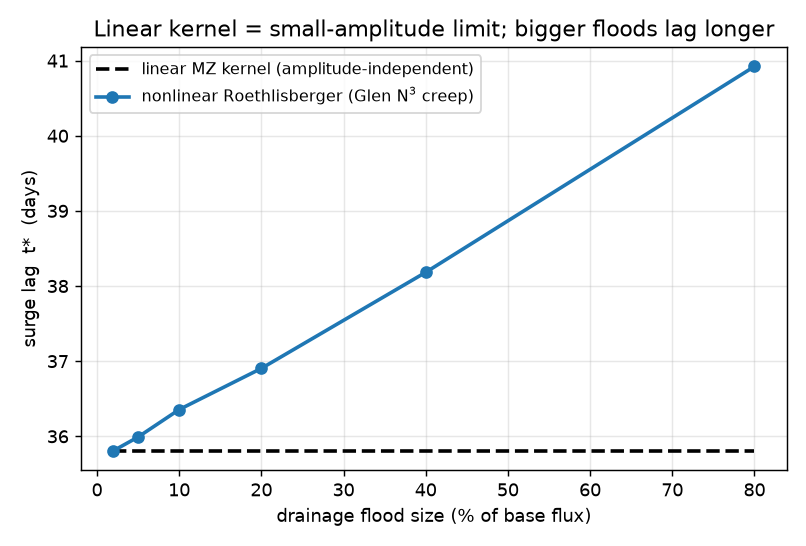
\includegraphics[width=0.82\linewidth]{figures/77_hydraulic_nonlinear_kernel.png}
\caption{Surge lag $t*$ versus drainage flood size in the nonlinear Röthlisberger cavity\ensuremath{\leftrightarrow}channel model. The linear Mori–Zwanzig kernel (dashed) is amplitude-independent and equals the nonlinear lag in the small-flood limit; the Glen-law $N^{3}$ creep closure makes the nonlinear lag (circles) rise with flood size — bigger floods lag longer, a falsifiable prediction the linear kernel cannot make.}
\end{figure}


\textbf{4.5 The kernel survives spatial resolution: a distributed operator projection whose no-transport limit is the lumped 2\ensuremath{\times}2.} The other half of the ``2\ensuremath{\times}2 identity'' objection is \emph{spatial}: a lumped two-box model has no geometry, so is the memory kernel an artefact of collapsing the drainage line to a point? We resolve the flowline. Take the linearised cavity\ensuremath{\leftrightarrow}channel system as two coupled \emph{fields} on a 1-D flowline — $\partial _{t}s = D_{s} \partial ₓₓs - s/\tau _{1} - a q$ (cavity store $s$) and $\partial _{t}q = D_{q} \partial ₓₓq - U \partial ₓq + b s - q/\tau _{2}$ (the channel $q$, which \emph{routes water downstream} at speed $U$ and spreads it at $D_{q}$; Röthlisberger 1972; Werder et al. 2013) — and project out the channel \emph{field} exactly (linear Nakajima–Zwanzig). The resolved store obeys a generalized Langevin equation $\dot{s} = A_{ss} s + \int _{0}^{t} 𝒦(t-\tau ) s(\tau ) d\tau  + R$ whose kernel $𝒦(\tau ) = A_{sq} e^{A_{qq} \tau } A_{qs}$ is now a \emph{matrix-valued, spatially non-local} operator. On $N=24$ flowline nodes (\code{validation/\allowbreak{}synthetic/\allowbreak{}hydraulic\_\allowbreak{}mz\_\allowbreak{}spatial.\allowbreak{}py}, 6 tests): (i) the projection is \textbf{exact} — the GLE transfer operator equals the full resolvent's resolved block at random complex $s$, max rel-err $7\times 10^{-16}$; (ii) the kernel \textbf{is} the eliminated channel operator's Green's function ($3\times 10^{-17}$ vs $expm$) and is spatially non-local with a resolved along-flow range $\ell _{mem}\approx 0.31 \gg  \Delta x$; (iii) the channel-eliminated field-GLE reproduces the full PDE trajectory ($1\times 10^{-5}$); and (iv) memory necessity is a \textbf{dose-response} — the memoryless local closure's trajectory error grows monotonically with the channel time $\tau _{2}$ and vanishes as $\tau _{2}\to 0$ (the Markovian limit, now derived \emph{in the distributed system}). Crucially, \textbf{the committed lumped 2\ensuremath{\times}2 kernel is exactly this projection's no-transport, single-node limit}: with $D_{q}=U=0$ the operator kernel $𝒦(\tau )$ is exactly diagonal and its diagonal equals $-ab e^{-\tau /\tau _{2}}$ to $7\times 10^{-18}$. Switching channel transport on moves the kernel mass off-diagonal (off-diagonal fraction $0\to 0.99$), so the surge-lag memory acquires a finite \textbf{along-flow footprint} with the closed-form decay length $\ell _{mem} = 2D_{q}/(\sqrt{U^{2}+4D_{q}/\tau _{2}}-U)$ (verified against the numeric steady-influence operator to $4\times 10^{-4}$; \emph{ballistic} limit $\ell _{mem}\to U\tau _{2}$ for fast channels, \emph{diffusive} limit $\ell _{mem}\to \sqrt{D_{q}\tau _{2}}$ for $U\to 0$) — a new, falsifiable, \textbf{field-measurable} structural prediction: a drainage's lagged velocity response is spread along the flowline over $\ell _{mem}$, which a memoryless (local) closure sets to zero. This converts the 2\ensuremath{\times}2 ``identity'' into the spatially-local limit of an exact projection of a genuine distributed (PDE) operator. Scope: still a \emph{linearised} distributed model on a periodic flowline; the fully nonlinear spatially-resolved coupled PDE remains future work.


\begin{figure}[htbp]
\centering

\includegraphics[width=0.82\linewidth]{figures/78_hydraulic_mz_spatial.png}
\caption{The distributed cavity\ensuremath{\leftrightarrow}channel memory kernel $𝒦(\tau =\tau _{2})$ (left) is spatially non-local — the off-diagonal band is the downstream channel transport that the lumped 2\ensuremath{\times}2 omits; its along-flow influence profile (centre) has a finite memory range $\ell _{mem}\approx 0.31$ versus the lumped kernel's zero-range spike; and the memoryless local-closure trajectory error (right) grows with the channel relaxation time $\tau _{2}$, vanishing in the Markovian ($\tau _{2}\to 0$) limit.}
\end{figure}


\medskip\hrule\medskip


\section*{5. The matched lag test — an honest null}


Both halves of a matched test are open: drainage \textbf{dates} from CryoSat-2 in-lake elevation ($detect_{drainages}$ extracts 7 fill\ensuremath{\to}drain events across 5 lakes, including the documented Mercer \ensuremath{\approx}2012.5 drainage), and velocity \textbf{response} from ITS\_LIVE box-mean surface speed.


\begin{center}\small
\begin{tabularx}{\linewidth}{>{\raggedright\arraybackslash}X>{\raggedright\arraybackslash}X>{\raggedright\arraybackslash}X>{\raggedright\arraybackslash}X>{\raggedright\arraybackslash}X>{\raggedright\arraybackslash}X}
\toprule
lake & base speed (m/yr) & drainages & annual noise floor & quarterly scatter & peak post-drainage \\
\midrule
Mac1 & 422 & 3 & 1.0\% & 2.3\% & \textbf{+0.56\ensuremath{\sigma}} \\
Mac2 & 402 & 1 & 1.1\% & 2.1\% & +0.27\ensuremath{\sigma} \\
Mac3 & 394 & 1 & 1.1\% & 3.4\% & -0.12\ensuremath{\sigma} \\
\bottomrule
\end{tabularx}
\end{center}


\textbf{Result.} No matched lake shows a post-drainage surge above the 2\ensuremath{\sigma} floor (peak $+0.56\sigma $, 0/5 significant). The lag value stays \emph{not} promoted to.


\textbf{Why null is a \emph{stronger} statement than ``too noisy''.} The modern ITS\_LIVE record is well resolved (annual \ensuremath{\approx}1 \%, quarterly \ensuremath{\approx}2–3 \%), so the limit is not a noise budget. Two distinct, quantifiable limits remain: (1) \textbf{temporal aliasing} — the derived lag is sub-annual ($t*$ baseline \ensuremath{\approx}0.01 yr, p95 \ensuremath{\approx}0.1 yr), finer than the finest \emph{robust} ITS\_LIVE bin (quarterly, 0.25 yr); a brief transient is averaged out regardless of scatter (a Nyquist limit); (2) \textbf{amplitude bound} — a \emph{sustained} speed-up would survive aliasing as a step, yet the peak anomaly is only $+0.56\sigma $, bounding any sustained surge to \ensuremath{\lesssim}10 m/yr on \textasciitilde{}400 m/yr. These map onto the two routes to a verified lag: \textbf{sub-annual GPS/GNSS} (EarthScope/POLENET; beats aliasing) \textbf{or fast-outlet trunk velocity} (e.g. Byrd, Stearns et al. 2008; steep $v(N)$ sensitivity beats the amplitude floor), paired with that site's drainage dates.


\textbf{Vetted forcing obtained.} USAP-DC 601439 (Smith et al. 2009 ICESat) yields \textbf{58 drainage events across 52 lakes} (median drained volume 0.128 km\ensuremath{^{3}}, max 2.92 km\ensuremath{^{3}}; implied water flux $q_{water}$ median \ensuremath{\approx}2.5 m\ensuremath{^{3}}/s, p95 \ensuremath{\approx}31 m\ensuremath{^{3}}/s — squarely in the literature subglacial-flood range), anchoring the §3/§4 forcing magnitude to real observations.


\medskip\hrule\medskip


\section*{6. A continental intrusion screen: RTN is the flotation ratio, and its only escape}


\textbf{6.1 Definition.} $RTN = (p_{ocean} - p_{atm})/p_{w}$ on grounded ice: overburden $p_{i}=\rho _{i} g H$, ocean head at the bed $p_{ocean}=\rho _{w} g\cdot d_{base}$ ($d_{base}=max(0,-bed)$), subglacial water $p_{w}=\phi  p_{i}$ (so $N_{eff}=(1-\phi )p_{i}$), gauge-corrected so the atmosphere cancels ($p_{atm}=0$). Then $RTN = \rho _{w} d_{base}/(\phi  \rho _{i} H)$, so `RTN>1 \ensuremath{\iff} \ensuremath{\rho}\_w d\_base/(\ensuremath{\rho}\_i H)

\begin{quote}
\ensuremath{\phi}$ — the ice is within a factor $\ensuremath{\phi}$ of flotation ($N\ensuremath{\to}0`; Schoof 2007; Leguy et al.
\end{quote}

2014; Cuffey \& Paterson 2010). \textbf{$RTN$ is, by construction, a nondimensional form of the flotation/effective-pressure criterion, not an independent predictor.}


\textbf{6.2 Result on Bedmap2.} Over 1.33 M grounded cells (1 km decimated to 3 km, $\phi =0.9$), the $RTN>1$ fraction decays monotonically with distance to the grounding line (15.1 \% within 5 km \ensuremath{\to} 0 \% beyond 100 km; median distance 6 km for $RTN>1$ cells vs 222 km for the rest), and the directional result reproduces on the independent \textbf{BedMachine v4} (NSIDC-0756) inversion (median 6 km vs 200 km to the grounding line).


\textbf{6.3 No skill over thickness-above-flotation (constant $\phi $).} A direct baseline test on 478,767 grounded Bedmap2 cells confirms ${RTN>1}$ is \emph{identical} to the thickness-above-flotation threshold ${H_{af}/H<1-\phi }$ (agreement \textbf{100.0000 \%}, 0 disagreeing cells, $\phi =0.8/0.9/0.95$), with $Spearman(RTN, H_{af}/H)=-1.000$ — so at constant $\phi $, $RTN$ \textbf{adds no skill}; it \emph{is} that standard quantity, nondimensionalised by $\phi $ (\code{validation/\allowbreak{}external/\allowbreak{}rtn\_\allowbreak{}baseline\_\allowbreak{}skill.\allowbreak{}py}).


\textbf{6.4 The only escape — a data-derived $\phi (x,y)$.} Because $RTN=(1-H_{af}/H)/\phi $ is algebraically forced to track the flotation fraction at constant $\phi $, $RTN$'s only possible independent signal is $\phi $ \emph{itself}. A synthetic plant-and-recover (\code{validation/\allowbreak{}synthetic/\allowbreak{}rtn\_\allowbreak{}variable\_\allowbreak{}phi\_\allowbreak{}skill.\allowbreak{}py}, 5 tests) shows a connectivity-informed $\phi (x,y)$ adds genuine skill over thickness-above-flotation (near-flotation-band $F1$ 0.78\ensuremath{\to}0.89; $AUC$ 0.995\ensuremath{\to}0.999), a random $\phi $ of the same distribution adds none, and the gain rises monotonically with $\phi $'s informativeness. On real Bedmap2, a calibration-free $\phi (x,y)$ from subglacial hydraulic-potential routing (Shreve 1972: priority-flood fill + D8 flow accumulation) reproduces the constant-$\phi $ anchor exactly and then reorders the intrusion class on \textasciitilde{}10\ensuremath{^{3}} near-grounding-line cells (near-flotation-band $Spearman$ $-0.99$ vs $-1.00$), nearly rank-independent of the flotation fraction in-band (\code{validation/\allowbreak{}external/\allowbreak{}rtn\_\allowbreak{}variable\_\allowbreak{}phi\_\allowbreak{}real.\allowbreak{}py}). The reordering is real but its \emph{correctness} is unvalidated — the routed $\phi $ is a model field derived from the same geometry — so the decisive test needs a $\phi $ from an \textbf{independent} observation of basal water (radar bed specularity; Schroeder et al. 2013, 2015), scored against a future gridded intrusion survey. We thus present variable-$\phi $ $RTN$ as a falsifiable screen with one clearly-stated open data step, not a verified forecast.


\textbf{6.5 Intrusion residence number $Ro$.} The level-set advance speed of the $RTN=1$ front is $v_{kin}=A\cdot dH/dt$; the residence number $Ro=v_{kin}\cdot \tau _{hyd}/\ell $ (regime boundary $Ro=1$ at the critical residence $\tau _{crit}=\ell /v_{kin}$) predicts whether intrusion is thinning-paced ($Ro\approx 1$) or hydraulic-limited ($Ro\gg 1$). For the runaway-tail cells ($A=0.70 km/m$, $dH/dt=1.5 m/yr$) \textasciitilde{}98 \% of the §4 residence band lies below $\tau _{crit}\approx 1.9 yr$ \ensuremath{\Rightarrow} predicted \textbf{thinning-paced}; a DInSAR $v_{obs}$ would place it on the curve (\code{validation/\allowbreak{}synthetic/\allowbreak{}intrusion\_\allowbreak{}residence\_\allowbreak{}number.\allowbreak{}py}, 7/7 tests).


\textbf{6.6 One state variable behind three thresholds (a derived unifier).} Height above flotation $h_{af}=H-H_{f}$ (with $H_{f}=(\rho _{w}/\rho _{i})d_{base}$; Schoof 2007) ties the three thresholds this framework treats separately into one. The ocean-connected effective pressure is $N=\rho _{i}g\,h_{af}$ \emph{exactly} (so $N=0\iff h_{af}=0\iff $ flotation); the $RTN=1$ intrusion surface is $h_{af}=H(1-\phi )$, which $\to 0$ as $\phi \to 1$ (the intrusion surface \emph{is} the flotation surface once subglacial water reaches overburden); and the sliding-law $|s_{N}|$ pole (Paper 4b) sits at $h_{af}^{c}=N_{c}/(\rho _{i}g)>0$, a few metres \emph{above} geometric flotation. A thinning stream therefore reaches the drag-side fold (the velocity early-warning) \emph{first} and ungrounds ($h_{af}\to 0$) only later --- a buffer set by $N_{c}$. RTN, the Schoof saddle-node, and the $s_{N}$ pole are thus three readings of one state variable, not independent diagnostics (verified on a synthetic thinning sweep: $N=\rho _{i}g\,h_{af}$ to machine zero, $h_{af}^{c}=6.67$ m; \code{nr10\_\allowbreak{}flotation\_\allowbreak{}unifier}).


\medskip\hrule\medskip


\section*{7. Estimator calibration (synthetic plant-and-recover)}


Every real-data estimator has a synthetic null/recovery harness exercised in \code{pytest}:


\begin{itemize}
\item \textbf{Lag estimator is kernel-shape-generic} — plant one target lag with five markedly different causal kernels (Gamma $k=2/4$, log-normal, bi-exponential, raised-cosine); $estimate_{lag}$ recovers it to \ensuremath{\le}10 \% for every shape; a delta-kernel control returns 0.
\item \textbf{RTN classifier / $\phi $-area inversion / variable-$\phi $ skill} — planted thresholds and connectivity recovered without bias ($rtn_{synthetic}$, \code{rtn\_\allowbreak{}phi\_\allowbreak{}synthetic}, \code{rtn\_\allowbreak{}variable\_\allowbreak{}phi\_\allowbreak{}skill}).
\item \textbf{Grounding-line migration level-set law is exact} — $|dH/dt|/|\nabla m|$ reproduced to rel-err $5\times 10^{-16}$ (1-D) / $4\times 10^{-14}$ (tilted 2-D).
\item \textbf{MZ projection} — the five §4 properties to machine precision (\code{hydraulic\_\allowbreak{}mz\_\allowbreak{}projection\_\allowbreak{}synthetic}, 6/6).
\end{itemize}


\medskip\hrule\medskip


\section*{8. Discussion and limitations}


\textbf{What this is.} A machine-precision certification of the cavity\ensuremath{\leftrightarrow}channel kernel's exact MZ structure (the central positive result); a motivated null on a literal thermal sliding kernel; an honest matched-lag null with a precise diagnosis and a concrete unblock path; and a flotation-ratio intrusion \emph{screen} whose only genuine degree of freedom (a data-derived $\phi (x,y)$) is isolated and partially tested.


\textbf{What this is not.} No verified surge-lag \emph{value} (the matched test is null; the value is to order of magnitude only). The §4.4 nonlinear extension shows the linear kernel is the small-amplitude limit of the nonlinear \emph{lumped} Röthlisberger system and predicts an amplitude-dependent lag, and the §4.5 distributed extension certifies the kernel as an exact spatially non-local operator projection of the linearised flowline PDE; only the fully \emph{nonlinear spatially-resolved} coupled GlaDS/Röthlisberger PDE remains future work. No RTN precision/recall (no gridded survey). The physical distinctness of $\phi $ from the Leray pressure remains unproven.


\textbf{Open gates, each with a concrete unblock.} (1) Matched lag \ensuremath{\to} sub-annual GPS/GNSS or fast-outlet trunk velocity, paired with drainage dates. (2) The \emph{linear} distributed projection (§4.5) and the \emph{lumped} nonlinear extension (§4.4) are done; the remaining gate is the fully \emph{nonlinear spatially-resolved} coupled GlaDS/Röthlisberger PDE. (3) RTN skill \ensuremath{\to} a $\phi (x,y)$ from an independent basal-water observable (specularity) + a gridded intrusion survey.


\medskip\hrule\medskip


\section*{9. Reproduce}


\begin{Verbatim}
pip install -r requirements.txt
python glaciers/validation/external/run_sliding_real.py --with-velocity Mac1 # §3 τ_ice + ITS_LIVE
python -m glaciers.validation.external.lag_fit_real                          # §5 matched-lag null
python glaciers/validation/external/run_usapdc_lakes.py                      # §5 vetted forcing (58 events)
pytest glaciers/tests/test_validation_synthetic.py -v                        # §4 MZ projection (6/6) + §7
python glaciers/validation/external/rtn_baseline_skill.py --stride 5         # §6.3 RTN==flotation (zero skill)
python glaciers/validation/synthetic/rtn_variable_phi_skill.py               # §6.4 variable-φ is the only escape
python glaciers/validation/external/rtn_variable_phi_real.py --stride 10     # §6.4 hydraulic-routing φ(x,y)
python glaciers/validation/synthetic/intrusion_residence_number.py           # §6.5 residence number Ro
python glaciers/validation/synthetic/hydraulic_nonlinear_kernel.py            # §4.4 nonlinear kernel (linear = small-amplitude limit)
python glaciers/validation/synthetic/hydraulic_mz_spatial.py                  # §4.5 distributed projection (lumped 2×2 = no-transport limit)
\end{Verbatim}

\section*{Data and code availability}


All analysis code and derived products are in the public repository at https://github.com/abdh0saifelden2-debug/K, and the results regenerate from the scripts above. The study uses the following open datasets:


\begin{itemize}
\item Bedmap2 ice thickness (Fretwell et al., 2013, https://doi.org/10.5194/tc-7-375-2013).
\item Independent ice thickness and active-lake inventory: USAP-DC 601470 (Stubblefield et al., 2021, https://doi.org/10.15784/601470; ice thickness after Arthern et al., 2015; active lakes after Siegfried \& Fricker, 2018).
\item Active subglacial-lake drainage volumes: USAP-DC 601439 (Smith et al., 2012, https://doi.org/10.15784/601439; ICESat inventory of Smith et al., 2009).
\item BedMachine Antarctica v4 (Morlighem, 2025, https://doi.org/10.5067/POJQI54A45HX; see Morlighem et al., 2020) for the independent continental RTN screen.
\item ITS\_LIVE surface velocities (Gardner et al., 2025, https://doi.org/10.5067/JQ6337239C96; see Gardner et al., 2018) and CryoSat-2 lake-drainage dates.
\end{itemize}


USAP-DC data were obtained from the U.S. Antarctic Program Data Center (https://www.usap-dc.org); BedMachine and ITS\_LIVE from the NASA NSIDC DAAC.


\section*{References}


Arthern, R. J., Hindmarsh, R. C. A., \& Williams, C. R. (2015). Flow speed within the Antarctic ice sheet and its controls inferred from satellite observations. \emph{Journal of Geophysical Research: Earth Surface} 120(7), 1171–1188. doi:10.1002/2014JF003239


Cuffey, K. M., \& Paterson, W. S. B. (2010). \emph{The Physics of Glaciers}, 4th ed. Academic Press, Amsterdam.


Curl, R. L. (1966). Scallops and flutes. \emph{Transactions of the Cave Research Group of Great Britain} 7, 121–160.


Fretwell, P., Pritchard, H. D., Vaughan, D. G., et al. (2013). Bedmap2: improved ice bed, surface and thickness datasets for Antarctica. \emph{The Cryosphere} 7, 375–393. doi:10.5194/tc-7-375-2013


Gardner, A. S., Moholdt, G., Scambos, T., et al. (2018). Increased West Antarctic and unchanged East Antarctic ice discharge over the last 7 years. \emph{The Cryosphere} 12, 521–547. doi:10.5194/tc-12-521-2018


Gardner, A., Fahnestock, M., Greene, C. A., Kennedy, J. H., Liukis, M., Lopez, L., \& Scambos, T. (2025). MEaSUREs ITS\_LIVE Regional Glacier and Ice Sheet Surface Velocities, Version 2 (NSIDC-0776) [Data set]. \emph{NASA NSIDC DAAC.} doi:10.5067/JQ6337239C96


Hewitt, I. J. (2013). Seasonal changes in ice sheet motion due to melt water lubrication. \emph{Earth and Planetary Science Letters} 371–372, 16–25. doi:10.1016/j.epsl.2013.04.022


Leguy, G. R., Asay-Davis, X. S., \& Lipscomb, W. H. (2014). Parameterization of basal friction near grounding lines in a one-dimensional ice sheet model. \emph{The Cryosphere} 8, 1239–1259. doi:10.5194/tc-8-1239-2014


Morlighem, M., Rignot, E., Binder, T., et al. (2020). Deep glacial troughs and stabilizing ridges unveiled beneath the margins of the Antarctic ice sheet. \emph{Nature Geoscience} 13, 132–137. doi:10.1038/s41561-019-0510-8


Morlighem, M. (2025). MEaSUREs BedMachine Antarctica, Version 4 (NSIDC-0756) [Data set]. \emph{NASA National Snow and Ice Data Center DAAC.} doi:10.5067/POJQI54A45HX


Mori, H. (1965). Transport, collective motion, and Brownian motion. \emph{Progress of Theoretical Physics} 33, 423–455. doi:10.1143/PTP.33.423


Nakajima, S. (1958). On quantum theory of transport phenomena. \emph{Progress of Theoretical Physics} 20, 948–959. doi:10.1143/PTP.20.948


Nikuradse, J. (1933). Strömungsgesetze in rauhen Rohren. \emph{VDI-Forschungsheft} 361. (English transl. NACA TM 1292, 1950.)


Röthlisberger, H. (1972). Water pressure in intra- and subglacial channels. \emph{Journal of Glaciology} 11, 177–203. doi:10.3189/S0022143000022188


Schoof, C. (2007). Ice sheet grounding line dynamics: Steady states, stability, and hysteresis. \emph{Journal of Geophysical Research: Earth Surface} 112, F03S28. doi:10.1029/2006JF000664


Schoof, C. (2010). Ice-sheet acceleration driven by melt supply variability. \emph{Nature} 468, 803–806. doi:10.1038/nature09618


Schroeder, D. M., Blankenship, D. D., \& Young, D. A. (2013). Evidence for a water system transition beneath Thwaites Glacier, West Antarctica. \emph{Proceedings of the National Academy of Sciences} 110(30), 12225–12228. doi:10.1073/pnas.1302828110


Schroeder, D. M., Blankenship, D. D., Raney, R. K., \& Grima, C. (2015). Estimating subglacial water geometry using radar bed echo specularity: Application to Thwaites Glacier, West Antarctica. \emph{IEEE Geoscience and Remote Sensing Letters} 12(3), 443–447. doi:10.1109/LGRS.2014.2337878


Shreve, R. L. (1972). Movement of water in glaciers. \emph{Journal of Glaciology} 11, 205–214. doi:10.3189/S002214300002219X


Siegfried, M. R., Fricker, H. A., Carter, S. P., \& Tulaczyk, S. (2016). Episodic ice velocity fluctuations triggered by a subglacial flood in West Antarctica. \emph{Geophysical Research Letters} 43, 2640–2648. doi:10.1002/2016GL067758


Siegfried, M. R., \& Fricker, H. A. (2018). Thirteen years of subglacial lake activity in Antarctica from multi-mission satellite altimetry. \emph{Annals of Glaciology} 59, 42–55. doi:10.1017/aog.2017.36


Siegfried, M. R., \& Fricker, H. A. (2021). Illuminating active subglacial lake processes with ICESat-2 laser altimetry. \emph{Geophysical Research Letters} 48, e2020GL091089. doi:10.1029/2020GL091089


Smith, B. E., Fricker, H. A., Joughin, I. R., \& Tulaczyk, S. (2009). An inventory of active subglacial lakes in Antarctica detected by ICESat (2003–2008). \emph{Journal of Glaciology} 55, 573–595. doi:10.3189/002214309789470879


Smith, B., Fricker, H., Joughin, I., \& Tulaczyk, S. (2012). Antarctic Active Subglacial Lake Inventory from ICESat Altimetry. \emph{U.S. Antarctic Program Data Center.} doi:10.15784/601439


Stearns, L. A., Smith, B. E., \& Hamilton, G. S. (2008). Increased flow speed on a large East Antarctic outlet glacier caused by subglacial floods. \emph{Nature Geoscience} 1, 827–831. doi:10.1038/ngeo356


Stubblefield, A. G., Arthern, R. J., Kingslake, J., \& Siegfried, M. R. (2021). Antarctic ice thickness, slipperiness, and subglacial lake locations. \emph{U.S. Antarctic Program Data Center.} doi:10.15784/601470


Werder, M. A., Hewitt, I. J., Schoof, C. G., \& Flowers, G. E. (2013). Modeling channelized and distributed subglacial drainage in two dimensions. \emph{Journal of Geophysical Research: Earth Surface} 118, 2140–2158. doi:10.1002/jgrf.20146


Wingham, D. J., Francis, C. R., Baker, S., et al. (2006). CryoSat: A mission to determine the fluctuations in Earth's land and marine ice fields. \emph{Advances in Space Research} 37, 841–871. doi:10.1016/j.asr.2005.07.027


Zwanzig, R. (1960). Ensemble method in the theory of irreversibility. \emph{The Journal of Chemical Physics} 33, 1338–1341. doi:10.1063/1.1731409


Zwanzig, R. (1973). Nonlinear generalized Langevin equations. \emph{Journal of Statistical Physics} 9, 215–220. doi:10.1007/BF01008729


\end{document}
